\section{Configuration}
\label{sec:col}

% TODO Define configuration and which constructs we want to be configurable

\subsection{Motivation}

From observation 2 we saw that most configuration was done via the inclusion of
source code. This source code would expose constants (read: literal values
\emph{and} identifiers). The included source code, however, can do anything
that Jolie source normally can, and isn't limited to just the desired
configuration. As a result, a service developer cannot be certain that the
configurator (entity who provides configuration) doesn't start messing with
other details of the program. Deploying defensive
programming\footnote{Defensive programming techniques are usually employed for
systems that require high availability, or where safety and security is
required.} techniques against this becomes significantly more problematic,
since no guarantees about the configuration source file can really be made.

Distributing re-useable packages is also problematic with this approach.
Several features of package management requires that the package remains
read-only. For example, updating of packages require this, without it
source-code merges would be required.

We also saw that a lot of issues, that should have been a deployment issue,
became a code issue.

This gives us plenty of reason to explore the need for a native configuration
format.  Most other systems would most likely go for a system defined in user
code, as opposed to natively. An example of such framework, could be Vert.x, it
is a tool-kit for building reactive applications on the JVM.  Examples of such
``reactive applications'' are microservices. The configuration workflow is
shown in Figure \ref{fig:normal_conf}. The system will retrieve, and read
external configuration files, directed by the user code, and apply the
configuration as needed.

% Most other systems can do this at run time
% For example Vert.x does this by reading external configuration files
% Once configuration is done, we can start up the server

\begin{listing}[H]
\begin{minted}{text}
+------------------+     +-------------------+     +--------------------+
| executable start | --> | retrieve conf     | --> | read conf files    |
+------------------+     +-------------------+     +--------------------+
                                                             |
                            +-----+                          |
                            |     | reconfigure              |
                            |     v                          v
                         +-------------------+     +--------------------+
                         | server running    | <-- | perform conf       |
                         +-------------------+     +--------------------+
\end{minted}
\caption{Simplified workflow for configuration of Vert.x applications}
\label{fig:normal_conf}
\end{listing}

% http://vertx.io/blog/vert-x-application-configuration/
% http://vertx.io/docs/vertx-config/kotlin/

TODO Defined deployment time somewhere

However implementing such as a system in Jolie has its problems, most of these
come from the difference between general-purpose programming languages and
specialized programming languages.

In general-purpose languages, the constructs (such as a server's socket) for
the microservice architecture are created in user code. As a result they are
entirely accessible from user code. This make it feasible to change their
behaviour, since code can run before deployment occurs.

In Jolie the constructs are managed directly by Jolie. Doing this has multiple
advantages, such as less complexity in user code, but it also means that user
code is capable of doing less. Jolie user code can for example not control
networking directly, but is instead forced to use the abstractions provided by
Jolie (sending messages). The language puts constraints on certain
constructs being fully prepared directly in the source code. This is analogous
to a programming language requiring the types of a struct's field to be present
at compile time. As a result, not all constructs can be changed at run time.
Concrete examples of this includes the input ports, which needs to be ready at
deployment time. Thus without native support for configuration of these, it
would not be possible to change the input port.

\subsection{Configuration Units}
\label{sec:conf_units}

A configuration unit is the basic entity, which encapsulates the configuration
of a single Jolie module. A configuration unit is known by its name (known as
its ``profile''), along with which module it configures. Having multiple profiles
for the same module can be useful for a variety of use-cases. A common
use-case, could for example be to have separate profiles for development and
production.

The units hold configuration for every possible type of configurable construct
in Jolie. The ones supported are:

\begin{enumerate}
    \item Input and output ports
        \begin{itemize}
            \item Location
            \item Protocol and protocol parameters
            \item Embedding of other services (output ports only)
        \end{itemize}
    \item General purpose parameters (constant values accessible from
            Jolie programs)
    \item Interface rebinding
\end{enumerate}

In the coming sections we'll mostly focus on the first two, in Section
\ref{sec:interface_rebinding} we'll cover interface rebinding.

% TODO Do we allow for inclusion of other files?
Configuration units are defined in configuration files, which may contain
several units. These files may even include other files, to pull in more
configuration units.

Jolie provides a new configuration file format. This format is custom, and made
to mimic the syntax of Jolie. Listing \ref{lst:simple_conf} shows a very
simple configuration unit. This units sets the location and protocol for the
output port \joliel{A}, the location of the input port
\joliel{ModuleInput}, and a parameter.

\begin{listing}[H]
\begin{minted}{jolie}
profile "hello-world" configures "my-module" {
    outputPort A {
        Location: "socket://a.example.com:3000"
        Protocol: sodep { .keepAlive = true }
    },

    inputPort ModuleInput {
        Location: "socket://localhost:80"
    },

    myParameter = 42,
    myParameter.subProperty = "hello"
}
\end{minted}

\caption{A simple configuration unit named \joliel{hello-world}
    configuring the module \joliel{my-module}}

\label{lst:simple_conf}

\end{listing}

Embedding of output ports can be performed from within a configuration unit.
This moves the embedding from being a code problem to, what it should have
been, a deployment problem. Listing \ref{lst:conf_embedding} shows the
embedding of output port \joliel{A}. Note that we need to make a
reference to the module, since the profile names are placed under a namespace
for each module. This way multiple services can share the same name, a
situation which is likely to occur with common profile names, such as
``development'' and ``production''.

\begin{listing}[H]
\begin{minted}{jolie}
profile "hello-world" configures "my-module" {
    outputPort A embeds "a-module" with "a-profile"
}

profile "a-profile" configures "a-module" {
    // configuration of a-module goes here.
}
\end{minted}
\caption{Embeddings make reference to other configuration units}
\label{lst:conf_embedding}
\end{listing}

As we can see from the examples, it is not necessary to provide all the values
of a port. It isn't necessary for two reasons. The first reason is that certain
values may be provided by the underlying module, which uses this unit. If a
module provides a value, then the configuration unit cannot override it. The
second reason is that configuration profiles may extend other profiles.

Configuration units may extend another unit, which configures the same module.
The tree of inheritance may be of an arbitrary depth, but each unit may only
extend a single unit, and they must configure the same module. The child is
also wins when it comes to configuration. This means that if unit ``B'' extends
``A'', and they both configure the same value, then the values found in B is
the one that is correct. Listing \ref{lst:conf_extends} shows an example of
extension with units.

\begin{listing}[H]
\begin{minted}{jolie}
profile "a" configures "a-module" {
    aValue = 42,
    aValue.sub = "hello",

    outputPort ExternalService {
        Location: "socket://external.example.com:42000"
    }
}

profile "b" configures "a-module" extends "a" {
    aValue = 100
    // aValue.sub = "hello"
    // ExternalService.location = "socket://external.example.com:42000"
}
\end{minted}
\caption{Configuration units may extend other units}
\label{lst:conf_extends}
\end{listing}

The module developer is often aware of what the defaults should be. For this
reason default configuration profiles may be shipped along the modules, which
are implicitly imported into every configuration file. The Jolie engine will
look for any \txtl{.col} file\footnote{The file extension of the
configuration file} in the \txtl{conf} folder. This folder
should be placed relative to the module's root. For example, if module "a" has
a file called \txtl{conf/my-defaults.col}, which contains a unit
called "default". Then the user of the package may either write a configuration
unit which extends this, simply by writing \joliel{profile
"something" configures "a" extends "default"}, or the default
directly. There is no need for any inclusion of this file.

It should be noted that no single unit is required to provide all
configuration. The system doesn't have any ``abstract''\footnote{As in abstract
classes, a concept often used in object oriented programming} configuration
units. However it is required that the configuration file provides all the
necessary configuration, as declared by the module. We'll learn more about
how a module declares configuration in Section \ref{sec:ol_conf}.

\subsection{Configuration and the Core Language}
\label{sec:ol_conf}

In section \ref{sec:conf_units} we learned about the configuration files, but
never actually saw the corresponding Jolie modules. In this section we'll
discover how the language has changed to accommodate this configuration
feature.

TODO The overall goals of the configuration system is:

\begin{itemize}
\item Easily identify the configuration possibilities of a module
\end{itemize}

\subsubsection*{Input and Output Ports}

% TODO Need to clean this up.
%
% 1. Present solution
% 2. Discuss problems

Input and output ports, both existing constructs, are defined just like before
in the Jolie code. To understand how the configuration system works with Jolie
code, it is important to first understand the subtleties of the pre-existing
system. TODO Input ports require that all fields are defined at deployment
time. Output ports require only the interfaces to be pre-defined, both the
location and protocol can be rebound and run-time.

In order to make a port externally configurable you simply define the port like
you normally would, and leave out the fields that should be configurable.
Listing \ref{lst:configurable_input} shows a configurable input port. Only
fields which are not already listed become configurable. This is particularly
useful when building a service which needs to make assumptions about its input
ports. For example if a developer is building a generic web-server, it is
useful to allow the developer to change the location, but the protocol should
be fixed.

One typical assumption that Jolie services make about their input ports come
from aliases that are made in the protocol configuration, an example is shown
in line 4 of Listing \ref{lst:configurable_input}. The pointer statement takes
two variable paths, and makes the one on the left link to the one on the right.
The result of this pointer alias is that any operation running from that input
port will be able to set the variable \txtl{statusCode} and the status code of
the HTTP request will be set appropriately. It should also be noted that the
configuration units \emph{do not} support aliases, and there are no other ways
of accessing variables hidden in the protocol configuration. As a result any
service which needs to do something special with its protocol configuration,
like aliasing, must do it in source code. Since the aliased variable now also
takes on a new semantic meaning, it also makes sense that it must be named
directly in source code, and not left to configuration, where it could take
any arbitrary name.

\begin{listing}[H]
\begin{minted}{jolie}
inputPort MyWebServer {
    Protocol: http {
        .keepAlive = true;
        .statusCode -> statusCode;
    }
    Interfaces: MyWebServerInterface
}
\end{minted}
\caption{A bare-bones configurable input port for a web-server}
\label{lst:configurable_input}
\end{listing}

If instead, all values could be overwritten of a port then the underlying
service would not be able to make assumptions about the additional features
provided by, for example, its protocol. For this reason only values not
specified can be overwritten.

\subsubsection*{Parameters}

Parameters are read-only values which are provided to a Jolie program at
deployment time. A parameter is type-checked at deployment time, to ensure that
its type matches what the underlying service expects. Listing \ref{lst:params}
shows a parameter definition and its use.

The type-checking feature functions both as a mean of documentation and
ensuring that the supplied configuration is valid. Like any other type-checked
feature of Jolie, it is possible to opt-out simply be setting the type to be
\txtl{undefined}.

\begin{listing}[H]
\begin{multicols}{2}
\begin{minted}[breaklines,fontsize=\footnotesize]{jolie}
// service.ol
parameters {
    myParameter: string {
       .foo: int
       .bar: bool
    }
}

main {
    println@Console(myParameter)(); // "Root"
    println@Console(myParameter.foo)(); // 42
    println@Console(myParameter.bar)() // false
}
\end{minted}

\columnbreak

\begin{minted}[breaklines,fontsize=\footnotesize]{jolie}
// service.col
profile "my-profile" configures "service" {
    myParameter = "Root",
    myParameter.foo = 42,
    myParameter.bar = false
}
\end{minted}

\end{multicols}
\caption{A parameter definition and its use}
\label{lst:params}
\end{listing}

From a high-level point of view, parameters are very similar to constants.
However parameters weren't implemented as an extension of constants due to
their technical implementation. Namely constants aren't implemented using the
``Value'' system, which is used by all variables and messages in Jolie, but
rather implemented at the parser level.

When the Jolie parser encounters a constant definition, it will save the token
from the assignment and associate it with the identifier on the left hand side.
Only identifier tokens and simple value tokens are allowed. The constant
definitions are limited to only a single token. As a result it isn't possible
to define more advanced tree-like values, which parameters such as
\joliel{myParameter} from Listing \ref{lst:params} would require.

Whenever the parser reaches a places where a constant would be allowed, it will
look at the next token, check if it is an identifier, and try to replace the
current token with the token defined by the constant. This produces some rather
surprising results and has limitations, which isn't commonly found in other
programming languages.  Listing \ref{lst:jolie_constants} illustrates how the
Jolie parser processes constants.

\begin{listing}[H]
\begin{multicols}{2}

\begin{minted}[breaklines,fontsize=\footnotesize]{jolie}
constants {
    FOO = 42
    BAR = ActualInterface
}

init {
    println@Console(FOO)()
}

courier Foo {
    [interface BAR(req)(res) {
        /* ... */
    }]
}
\end{minted}

\columnbreak

\begin{minted}[breaklines,fontsize=\footnotesize]{jolie}
init {
    println@Console(42)()
}

courier Foo {
    [interface ActualInterface(req)(res) {
        /* ... */
    }]
}
\end{minted}

\end{multicols}

\caption{Constants in Jolie works by replacing tokens at the parser level. Left:
    The input program. Right: The program which the parser ends up seeing}

\label{lst:jolie_constants}

\end{listing}

While it would have been possible to extend the value system to support values
it was ultimately decided against. Adding both optional type-checking of
constants and expanding to values was seen as too big a departure from the
original intent of constants. For backward compatibility reasons constants
would also still not have been pure values, but rather either an identifier or
a value.

The new parameters block is an addition to the AST of Jolie programs. This
addition currently only works in collaboration with the configuration and
module system. The block is simply not valid to use without. If any parameter
is not defined by configuration or has the wrong type the checking scripts of
Jolie will throw an error.

Even though the parameters block is added to the AST it will not be visible in
the final interpretation tree. We'll learn more about this in Section
\ref{sec:col_impl}.

\subsubsection*{Syntax Considerations}

TODO

This problem is however not without its problem, again consider Listing
\ref{lst:configurable_input}. Previously this code would have resulted in an
error from the semantic verification, specifically pointing out that an input
port must have its \joliel{Location} property set. This leads to the question
of how do we differentiate between code that is intended to be configurable and
code which is simply invalid.

TODO Discuss approaches to marking these

\subsection{Example}

TODO This is just copy pasted from some markdown document. Might be able to
find a better example. Syntax is most likely also outdated.

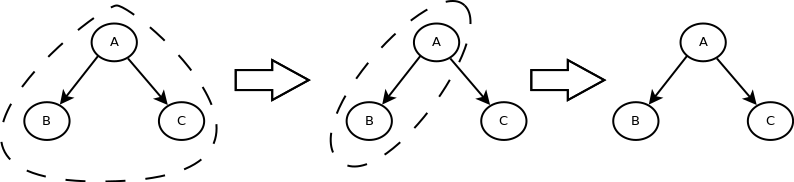
\includegraphics[width=\textwidth]{prototypes.png}

(The dashed region corresponds to which services that are embedded together)

This use-case is intended to show how we can easily go from a prototype where
we embed everything (this is easier to run locally) to hosting each service by
itself.

\begin{minted}{jolie}
// A.ol

ext outputPort A {
    Interfaces: AIface
}

ext outputPutPort B {
    Interfaces: BIface
}

constants {
    FOO: int
}
\end{minted}

\begin{minted}{jolie}
// A.col

include "B.col" // The includes work just like they do in Jolie
include "C.col"

// Previously called namespace. Configures makes it more explicit that we're
// talking about a specific package and not an arbitrary name
configures "A" {
    // Like always we just put the definitions here
    FOO = 42

    // We alter the syntax slightly for output ports being embedded
    outputPort B embeds B
    // The second B refers to the profile B (if no profile is specified it gets
    // the same name as the package it configures). This means that this
    // configures block also has name "A". It could also have been written as:
    // `profile "A" configures "A"`

    outputPort C embeds C
}
\end{minted}

Note: The previous proposal did not allow for embedding of services directly
from the configuration. This is however needed since packages by themselves
should be considered read-only. Thus if we want to configure a package to embed
its dependencies, then this must be done from external configuration, we cannot
do this in source.

\begin{minted}{jolie}
// B.col

configures "B" {
    inputPort B {
        Location: "local"
    }
}
\end{minted}

\begin{minted}{jolie}
// C.col

configures "C" {
    inputPort C {
        Location: "local"
    }
}
\end{minted}

In order to use an external B we need to update "A.col":

\begin{minted}{jolie}
// A.col
include "C.col"

configures "A" {
    outputPort B {
        Location: "socket://b.example.org:8000"
        Protocol: sodep
    }
    outputPort C embeds C
}
\end{minted}

In order to update the deployment file of B we simply need to update the
input port to no longer be local.

\begin{minted}{jolie}
// B.col
configures "B" {
    inputPort B {
        Location: "socket://localhost:8000"
        Protocol: sodep
    }
}
\end{minted}

In most cases however this would be unnecessary since the default
configuration file for "B" could already include a default input port.

In that case we could simply deploy directly from the default configuration.
The restriction on configuration units to only configure a single package helps
a lot. This restriction means that we cannot from any node configure any other
node which isn't a direct child of it. Without this we wouldn't be able to
easily swap out one configuration unit for another.

\section{Implementing the Configuration Format}
\label{sec:col_impl}

The new interpreter pipeline is as follows, new phases marked in bold text:

\begin{enumerate}
\item Intent parsing
\item Jolie code parsing
\item \textbf{Configurator}
\item Semantic verifier
\item Interpretation tree builder
\item \textbf{Late verification}
\item Communication core init
\item Init \& main process
\end{enumerate}

The primary work occurs in the configurator service, but some of the
verification work, namely the parameters, are postponed until after the
interpretation tree has been build.

\subsection{Syntax of the Configuration Format (COL)}

In this section the formal grammar of the configuration format is presented.
The grammar is presented in a ABNF-like syntax. Complete syntax is presented in
Appendix B.

All literals are case sensitive.

TODO is ABNF okay considering it is mostly used for communication protocols?

A configuration file starts by a list of includes, followed by a list of
regions.

\begin{minted}{abnf}
configuration-tree = *include *region

include = "include" qstring

region = region-header "{" region-body "}"
region-header = [ "profile" qstring ] "configures" qstring [ "extends" qstring ]
region-body = *definition
definition = port | interface | parameter
\end{minted}

The definitions inside of a region correspond to the different configurable
units. The syntax is made to closely mimic the syntax of existing Jolie code.

\begin{minted}{abnf}
port = input-port | output-port
input-port = "inputPort" identifier "{" port-body "}"
output-port = embedded-output-port | external-output-port
external-output-port = "outputPort" identifier "{" port-body "}"
embedded-output-port = "outputPort" identifier "embeds" qstring "with" qstring
port-body = *port-property
port-property = location-property | protocol-property
location-property = "Location" ":" qstring
protocol-property = "Protocol" ":" identifier [ protocol-config ]
protocol-config = inline-tree

interface = "interface" identifier "=" identifier "from" qstring

parameter = variable-path "=" value
variable-path = var-id *var-node
var-id = ( "(" qstring ")" ) | identifier
var-node = "." var-id [ "[" unsigned-int "]"  ]
value = ( primitive [ inline-tree ] ) | inline-tree
inline-tree = "{" *(tree-child ",") tree-child "}"
tree-child = "." variable-path "=" value
primitive = qstring | int | long | double | bool
\end{minted}

The values very closely resemble what Jolie allows, primarily just removing
variables from the syntax. Variable identifiers can be strings, like in Jolie,
to allow for special variable names which would otherwise not be
valid identifiers. This is primarily useful for building dictionary like
structures with arbitrary string keys.

Additional configuration file supports C-style comments, these are allowed
anywhere and are simply ignored.

\begin{minted}{abnf}
comment = single-line-comment | multi-line-comment
single-line-comment = "//" <any text except line breaks>
multi-line-comment = "/*" <any text except "*/"> "*/"
\end{minted}

\subsection{The Configuration Phase}

The configuration phase builds upon the result of the intent and parsing phase.
From the intent phase we receive information about modules and potentially
receive the intent to use a certain configuration unit. From the parsing phase
we obviously get the AST.

The configuration phase works by modifying the AST to insert the configuration
gathered from the configuration unit. The processed AST is handed to the later
phases, and the remainder of the pipeline works mostly like it has before.
% TODO Something about how only modifying the AST increases the likelihood of
% everything being okay, since for the remainder of the engine the
% configuration phase might as well not exist.

\subsubsection*{Processing of Configuration Files}

% Introduction

The first step of the configurator is to gather a fully processed configuration
unit. This process starts by looking for the configuration file which was
passed from the intent. The intent passes the configuration file using
\txtl{--conf <unitName> <fileName>}.

% File resolving

The configurator searches for the configuration file in TODO (parent services,
and example for this is needed).

% Parsing

With the configuration file resolved, it is passed to the configuration parser
along with a list of known modules. The parser follows the conventions
established by the existing Jolie code parser. The parser is a hand-written
recursive descent parser with one token lookahead.

The parser directly outputs the AST. At the top level the AST consists of
\javal{Region}s which directly map to the configuration unit abstraction. Each
\javal{Region} are namespaced under the module that they configure. Internally
each namespace maps the name of the \javal{Region} to the actual
\javal{Region}. The top-level node of the AST contains a dictionary mapping
between the name of modules and their namespaces. The Java type for this
mapping ends up being \javal{Map<String, Map<String, Region>>}, this allows for
easy access of \javal{Region}s when they are needed. This does however also
mean that duplicates must be caught during parsing, since they would otherwise
just silently override previous entries. This would typically have been
performed in a later stage to keep the parser ``pure''. In this case some
purity was sacrificed for some efficiency and ease of use.

The grammar of the configuration format closely follows the grammar of Jolie
code. As a result the configuration format also re-uses AST nodes where
possible. As we will see later, this proved helpful when outputting a
configured AST. The configuration grammar only supports a subset of the
features that Jolie code does.

Recall from Section \ref{sec:conf_units} that each module may publish default
configuration units, which can be used by user-level configuration units. For
this reason the parser will make special note of references to other
configuration units. Such references currently only appear in output port
embeddings (e.g. \\\joliel{outputPort Foo embeds "foo" with "a-foo-unit"}).

Once the initial file has been parsed, every single configuration file placed
in the ``conf'' directory of referenced modules are parsed and placed in the
same AST. Configuration files parsed during this phase may itself have
references to other modules, in that case these will be pulled in as well.  A
set of parsed defaults is kept to avoid parsing the same file multiple times,
or potentially infinite loops.

% Merging

With the entire configuration tree in place, merging is performed to create a
single \javal{Region} which represents the actual configuration. The merging
occurs between a \txtl{child} and its \txtl{parent} region (i.e. the one it
extends, if any) and results in a \txtl{merged} region. The \txtl{parent} is
always merged (via a recursive call) first. The first \txtl{child} selected is
the \txtl{Region} matching the profile name and package given by the intent.

For ports, the merging algorithm works by inserting all the ports of the
\txtl{child} into the \txtl{merged} region. The ports of the \txtl{parent} are
then merged with the preliminary output of the \txtl{merged} region. The
process of merging a \txtl{port} of the \txtl{parent} against the \txtl{merged}
region is shown, in pseudo code, in Listing \ref{lst:merge_ports}. In short the
merging will favor the \txtl{child}, and the \txtl{parent} will only provide
values if the \txtl{child} doesn't.

TODO Define what a partial configuration is

\begin{listing}[H]
\begin{minted}[linenos=true]{text}
procedure merge(port: Port, merged: ConfigTree): Region {
    if (!merged.contains(port)) return port
    existing = merged.getExisting(port)

    if (existing.isComplete) return existing
    // The existing port cannot be an embedding, since those cannot
    // be partial.

    for (property in Port.properties) {
        if (existing[property] == null) {
            existing[property] = merged[property]
        }
    }
    return existing
}
\end{minted}

\caption{Pseudo code for merging a \txtl{parent}'s \txtl{port} into a
    \txtl{merged} configuration tree}

\label{lst:merge_ports}

\end{listing}

For parameters the same idea applies. However each parameter definition node in
the AST potentially only provides a partial value. For example the node
\joliel{foo.bar = 42}, where the type of \joliel{foo} is \joliel{string { .bar:
int }}, only provides a partial definition of \joliel{foo}. For this
reason the parameter nodes are first added from the \txtl{parent} and then by
the \txtl{child}. This allows the definitions of the \txtl{child} to override
those of the \txtl{parent}.

\subsubsection*{Applying Configuration to the AST}

The \txtl{merged} region from the previous section is then used along
with the AST corresponding to the Jolie program being run. The last phase of
the configurator will process the entire AST and output a new AST, which is
fully configured. This process works by running a \txtl{process} function on
every single top-level node. The \txtl{process} function will inspect the node,
and depending on the node return a list of replacement nodes.

Throughout this process the configurator will also verify that no configuration
is performed on nodes which aren't configurable. This includes dynamic ports
and non-empty interface definitions.

\paragraph{Ports}

When a port node is encountered in the AST, the \txtl{merged} region is
searched for an output port matching its name. If none is found, the AST node
is returned as it is, no modifications are made to it. Otherwise the
configuration proceeds. For input ports and non-embedding output ports the
process is the same. The properties of the AST port and the port represented in
the configuration region are compared one-by-one. If any property is defined by
both, an error is returned pointing to the AST node and the place that the
configuration took place. At the end, if no errors are returned, a new port is
returned with their properties merged together.

For output ports which embed another module the process is slightly different.
The configurator will first verify the existence of the configuration unit by
looking it up in the configuration tree. If it is not found an error will be
returned. Otherwise the configurator will output a new embedding node. The
embedding node will contain a reference back to the same configuration file the
current \txtl{Region} comes from. When the embedding is performed, the
configurator of the embedded service will lookup the correct configuration unit
from the same file. This will however cause an addition parsing of the same
file, but a caching layer at the configuration parser could take care of this.
The embedding process is demonstrated in Listing \ref{lst:embedding_output}.

\begin{listing}[H]
\begin{multicols}{2}

\begin{minted}[breaklines,fontsize=\footnotesize]{jolie}
embedded {
    Jolie:
        "--conf foo-profile <inputConfigFile> foo.mod" in Foo
}
\end{minted}

\columnbreak

\begin{minted}[breaklines,fontsize=\footnotesize]{jolie}
outputPort Foo embeds "foo" with "foo-profile"
\end{minted}

\end{multicols}

\caption{AST nodes generated, shown as code (left), by configuration (right)
    for an output port containing an embedding}

\label{lst:embedding_output}

\end{listing}

\paragraph{Interface Rebinding}

Just like ports, when an interface definition is found the \txtl{merged} region
is searched for a matching interface definition. Assuming no errors, the
configurator must now replace the dummy interface definition with the real
interface definition as the configuration specifies.

Quickly recapping interface rebinding in the configuration is shown in Listing
\ref{lst:interface_rebinding_recap}. Note that the only information the
configurator has for locating the replacement is the name of the interface and
its module.

\begin{listing}[H]
\begin{minted}{jolie}
interface Dummy = Concrete from "my-module"
\end{minted}

\caption{Rebinding the interface \txtl{Dummy} to match the interface
    \txtl{Concrete} from the module \txtl{my-module}}

\label{lst:interface_rebinding_recap}

\end{listing}

The interface will be found by parsing the module's entry point. Its AST will
then be searched for an interface matching the replacement. Simply replacing
the dummy with its replacement, however, isn't enough. Consider, for example,
the scenario shown in Listing \ref{lst:interface_rebinding_types}. In this
scenario, the processed AST will no longer be valid due to the missing types
(\txtl{FooRequest} and \txtl{FooResponse}).

\begin{listing}[H]
\begin{minted}{jolie}
type FooRequest: void {
    .child: string
}

type FooResponse: int

interface Concrete {
    RequestResponse:
        foo(FooRequest)(FooResponse)
}
\end{minted}

\caption{Simply copying the interface definition is not enough, the types must
    also be copied}

\label{lst:interface_rebinding_types}
\end{listing}

The relevant type definitions are found by iterating through every operation of
the replacement interface. If the types listed in the operations are type links
those are followed. This leads to a recursive algorithm, which looks through
every type looking for type links, which will cause more types to be copied
over. In order to avoid infinite loops a set of already visited types is kept.
If a type has been seen before then its children will not be visited.

In the end, the original interface definition will be replaced, and all
necessary type definitions will also be added to the program.

\paragraph{Parameters}

Parameters being a new concept in Jolie simply outputs new nodes for every
single parameter assignment. This along with the definitions gathered from
ordinary Jolie code parsing are processed in interpretation building phase.

\subsection{Additions to the Semantic Verifier}

As discussed in Section \ref{sec:ol_conf} several syntax changes were also made
to the core languages. These modifications to the syntax also slightly changed
which programs were legal. As an example interfaces are now allowed to be empty
at a syntactical level, to signal that they should be replaced by
configuration. However having an empty interface not being replaced should
still cause an error.

This means that additional checking must not be performed to ensure that
programs are semantically valid. Such a phase already exists in the compiler,
the semantic verifier.

The semantic verifier works by performing an AST traversal and validate the
semantics of each node.

The verifier has been updated to not allow empty interfaces, this was
previously enforced at a syntax level. Since the configurator runs before this
phase and updates the AST, this will only cause errors for non-configured
trees.

Non-dynamic ports are ensured to be constant by using features already
implemented by the semantic verifier.

The semantic verifier is the last phase of the Jolie interpreter when run with
the \txtl{--check} flag. As we will discuss in the coming section, it is not
practical to perform type-checking of parameters at this point.

TODO Shouldn't the semantic verifier ensure that parameters are constant?

\subsection{Additions to the Interpretation Tree Builder and Late Verification}

% Introduction

Interpretation tree building was expanded to support parameters. All other
features required no changes to AST structure, and could simply reuse existing
features.

This section will discuss the technical of how the Interpretation Tree Builder
(ITB) works. It will cover issues that are quite technical, and very specific
to this particular implementation of the Jolie engine.

% What is the ITB and what does it do?

The Interpretation Tree Builder (ITB) is the last step before a Jolie program
is ready to be executed. The ITB works by traversing the AST. The ITB will
collect information from the AST in the form of definitions and inform the AST
about their presence. These definitions include ports, interfaces, types, and
code procedures.

% Processes

Within code procedures the ITB will produce processes from the AST nodes which
are runnable. It is from processes the meat of code execution is implemented.
For example it is from processes everything from addition to operation calls
are implemented.

% When are types ready?

In this phase the ITB will be gathering complete information about types. Type
building is for the most part a fairly trivial one-to-one translation from the
AST nodes into the internal type representation. The most important job of the
ITB with respect to type building is resolving of type references. This turns
references to a type name into an actual reference to a concrete internal type.
Because types aren't build until this phase is what makes type-checking during
semantic verification problematic. The semantic verifier would essentially have
to duplicate the work of the ITB in order to perform type-checking earlier.
This also means that type-checking cannot be performed until the ITB is
finished.

% State, and how the ITB changes initial state.

The ITB will need to initialize the system with certain values. For example,
the ITB will initialize the \joliel{location} and \joliel{protocol} variables
of output ports. These variables are local only to a single request. At this
point, however, the state of the Jolie program has not yet been initialized.

In Jolie, state is associated with the current thread of execution. Jolie uses
a separate thread of execution for handling every message. As a result every
single request gets its own fresh state. All state is copied from the
initialization execution thread. This thread performs work requested by the ITB
followed by the \joliel{init} procedure. Thus right after the ITB is done, and
the initialization execution thread is started, code execution starts. This
includes both user code in form of Jolie, but also loading of any embedded
services.

It should be noted that any process which works with state must be run on an
execution thread, since it depends on the state being present on the thread.

% Handling of parameter definitions and assignments inside the ITB

The ITB receives two new node types from the configurator and code parser:
parameter assignments, and parameter definitions.

For parameter definitions the ITB will resolve the types. Ensuring that all
links are properly resolved. This will output a ``processed'' parameter
definition which the ITB will inform the interpreter about.

In a similar fashion, the ITB will process parameter assignments and inform the
interpreter. Type-checking cannot be performed at this point, due to types not
being ready before the ITB finishes. Simply outputting processes for
configuration will make it impossible to perform type-checking before code
execution starts, due to their dependency on state.

The processed assignments contains an ordinarily processed LHS, which contains
the variable path. The RHS has been processed into an expression, which can be
evaluated into a native Jolie value on which type-checking can be performed.

% Introduction of new phase and working around lack of state

Because of these constraints a new ``late-checking phase'' has been created.
This phase runs right after the ITB, but before code execution starts. In this
phase it is not possible to directly touch the init state. It is however
possible to both create values, and evaluate expression. This phase creates a
synthetic state by creating a new value, which will act as the state.
Expression are evaluated against this root and later type-checked. The result
of evaluating the parameter assignments are then copied into the init state,
   assuming, of course, that type-checking was successful.

